\documentclass[10pt]{beamer}

%\usetheme{ENSLyon}

\usetheme{AnnArbor}

\title[CNMAC 2021]{\Large \textsc{Software HCprot:\\ Pré processamento de Instâncias Moleculares do Protein Data Bank}}
\author[G. Philippi]{{Guilherme Philippi\vspace{-0.3cm}}}
\institute[]{Departamento de Matemática\\ Universidade Federal de Santa Catarina, Blumenau \\ \vspace{0.2cm} Desenvolvido em conjunto com Felipe Fidalgo e Emerson V. Castelani\vspace{-0.2cm}}
\date[15 Setembro, 2021]{ {\small XL Congresso Nacional de Matemática Aplicada e Computacional} \\ {\scriptsize Minissimpósio 10 - Geometria de Distâncias e Álgrebras Geométricas\\ 15 de setembro de 2021}}
\setbeamersize{text margin left=5mm}
\setbeamersize{text margin right=5mm}

\setbeamertemplate{navigation symbols}{}
%\usecolortheme{ENSLyon_greener}
\usecolortheme{whale}

\setbeamercolor{frametitle}{bg=gray}
\setbeamertemplate{bibliography item}{\insertbiblabel}

%PACKAGES -------------------------
\usepackage{etex}
\usepackage[utf8]{inputenc}
\usepackage[brazilian]{babel}
\usepackage{enumerate}
\usepackage{amsmath}
\usepackage{amssymb}
\usepackage{amsthm}
\usepackage{amscd}
\usepackage{amsfonts}
\usepackage{multicol}
\usepackage{multirow}
\usepackage{array}
\usepackage{color}
\usepackage{graphicx}
\usepackage{tikz}
\usepackage{tikz-qtree}
\usepackage{wrapfig}
\usepackage{3dplot}
\usepackage{pgf}
\usepackage{tkz-euclide}
\usepackage{algorithmic}
\usepackage{algorithm}
\usepackage{xparse}
\usepackage{subfigure}

%LIBRARIES-TIKZ ------------------------------------------

\usetikzlibrary{shadows,trees}
\usetikzlibrary{decorations.pathmorphing}
\usetikzlibrary{decorations.markings}
\usetikzlibrary{positioning}
\usetikzlibrary{chains,matrix,scopes}
\usetikzlibrary{arrows}

%DEFINITIONS ----------------------------------------------------

\def\centerarc[#1](#2)(#3:#4:#5)% Syntax: [draw options] (center) (initial angle:final angle:radius)
{ \draw[#1] ($(#2)+({#5*cos(#3)},{#5*sin(#3)})$) arc(#3:#4:#5); }
\def\xx{\mathbf{x}}
\def\ii{\mathbf{i}}
\def\jj{\mathbf{j}}
\def\kk{\mathbf{k}}
\def\tt{\mathbf{t}}
\def\ee{\mathbf{e}}
\def\qq{\mathbf{q}}
\def\pp{\mathbf{p}}
\def\vv{\mathbf{v}}
\def\rr{\mathbf{r}}
\def\vzero{\mathbf{0}}
\def\qset{\mathbb{H}}
\def\xx{\mathbf{x}}


%\AtBeginSection[]
%{
%	\begin{frame}<beamer>
%		\frametitle{Inicio da seção \thesection}
%		\tableofcontents[currentsection]
%	\end{frame}
%}


%NEW THEOREMS ------------------------------------------

\theoremstyle{plain}
\newtheorem{teorema}{Teorema}[section]
\newtheorem{lema}{Lema}[section]
\newtheorem{proposicao}{Proposição}[section]
\newtheorem{corolario}{Corolário}[section]

\theoremstyle{definition}
\newtheorem{definicao}{Definição}[section]
\newtheorem{observacao}{Observação}[section]
\newtheorem{exemplo}{Exemplo}[section]

\newenvironment{solucao}
{\renewcommand\qedsymbol{$\triangle$}\begin{proof}[Solução]}{\end{proof}}



\begin{document}
	
	%FACE
	\begin{frame}
		
		\titlepage
		
		\vspace{-0.7cm}
		\begin{flushleft}
			
\includegraphics[scale=0.12]{logo.png}
		\end{flushleft}
		
		\vspace{-2cm}
		\begin{flushright}
			
\includegraphics[scale=0.024]{logo_ufsc.png}
		\end{flushright}
	\end{frame}
	
	%Indice
	\begin{frame}
		\tableofcontents 
	\end{frame}
	
	\section{Introdução}
	
	\begin{frame}
		\frametitle{\normalsize Worldwide PDB } 
		{
			\small
			
			\begin{center}
				
\includegraphics[width=0.4\linewidth]{wwpdb-logo.png}	
			\end{center}
			
			Todas as informações sobre a estrutura 3D de proteínas são concentradas no repositório Protein Data Bank (PDB) \cite{PDB}.
			
			\begin{center}
				\begin{minipage}{0.08\linewidth}
					\hspace{0.1cm}
				\end{minipage}	
				\begin{minipage}{0.4\linewidth}
					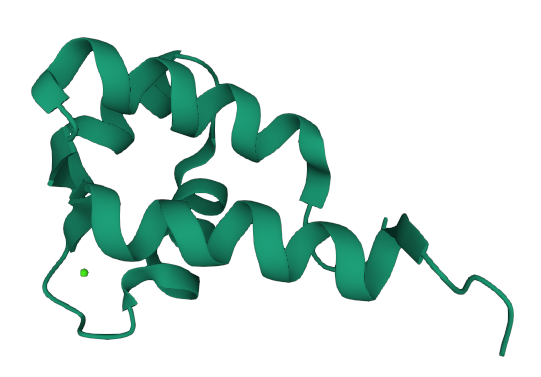
\includegraphics[width=0.8\linewidth]{prot2.png}
				\end{minipage}
				\begin{minipage}{0.08\linewidth}
					\hspace{0.5cm}
				\end{minipage}
				\begin{minipage}{0.4\linewidth}
					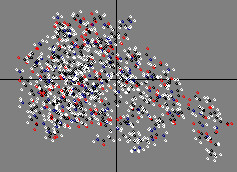
\includegraphics[width=0.7\linewidth]{prot.png}
				\end{minipage}
			\end{center}
		}	
	\end{frame}
	
	\begin{frame}
		\frametitle{\normalsize Geometria de Distâncias} 
		{
			\small
			\begin{definicao}[Distance Geometry Problem (DGP) \cite{carlileGDandAplications}]
				Dados um grafo simples, ponderado e conectado $G = (V, E, d)$ e um inteiro $K>0$, encontre uma realização $x: V \longrightarrow \mathbb{R}^K$ tal que:
				\begin{equation*}
					\forall \{u,v\} \in E, \hspace{0.5cm} \lVert x(u) - x(v) \rVert = d(\{u,v\}). \label{eq:DGP}
				\end{equation*}	
			\end{definicao}
		
			Chamamos $G$ de grafo DGP. Esse é um problema \textbf{NP}-completo para $K = 1$ e \textbf{NP}-difícil para $K>1$ \cite{Saxe:79}.
			\\
			
			\begin{definicao}[Discretizable Molecular DGP (DMDGP) \cite{carlile:MinimalOrder}]
				Dado um grafo DGP e uma ordenação nos vértices $v_1,\dots,v_n$ tal que
				\begin{itemize}
					\item Existe uma realização válida para $v_1, v_2, v_3$ e
					\item Para todo $i \geq 4$, o conjunto $\{v_{i-3}, v_{i-2}, v_{i-1}, v_i\}$ é um clique com $$d_{i-3,i-2} + d_{i-2,i-1} > d_{i-3,i-1},$$
				\end{itemize}
				encontre uma realização $x: V \longrightarrow \mathbb{R}^3$ tal que 
				$$\forall \{u,v\} \in E, \hspace{0.5cm} \lVert x(u) - x(v) \rVert = d(\{u,v\}).$$
			\end{definicao}
			}	
	\end{frame}
	
	\begin{frame}
		\frametitle{\normalsize Ordenação} 
		{
			\small
			Encontrar uma ordenação como a descrita no DMDGP é conhecido como Discretizable Vertex Ordering Problem (DVOP), que é de classe \textbf{P} para $K$ fixo \cite{douglasDVOP}. 
			\vspace{0.5cm}
			
			Também pode-se encontrar ordenações manualmente, se aproveitando de dados da estrutura 3D molecular, como a \textit{hand-crafted vertex order} (hc Order) \cite{carlile:MinimalOrder}:
			
			\begin{equation*}
				hc = \left\{ \quad N^1, H^1, H^{1'}, C_{\alpha}^1, N^1, H_{\alpha}^1, C^1, C_{\alpha}^1, \dots, \qquad \qquad \qquad \qquad \qquad \right.
			\end{equation*}%\vspace{-0.8cm}
			\begin{equation*}
				\qquad \qquad \ H^i, C_{\alpha}^i, O^{i-1}, N^i, H^i, C^{i}_\alpha, N^i, H^{i}_\alpha, C^i, C_{\alpha}^i,\dots, \qquad \qquad \qquad
			\end{equation*}%\vspace{-0.65cm}
			\begin{equation*}
				\left. \qquad \qquad \qquad H^p, C_{\alpha}^p, O^{p-1}, N^p, H^p, C^{p}_\alpha, N^p, H^{p}_\alpha, C^p, C_{\alpha}^p, O^p, C^p, O^{p'} \quad \right\},
			\end{equation*}
			
			\vspace{-2.2cm}
			\begin{center}
				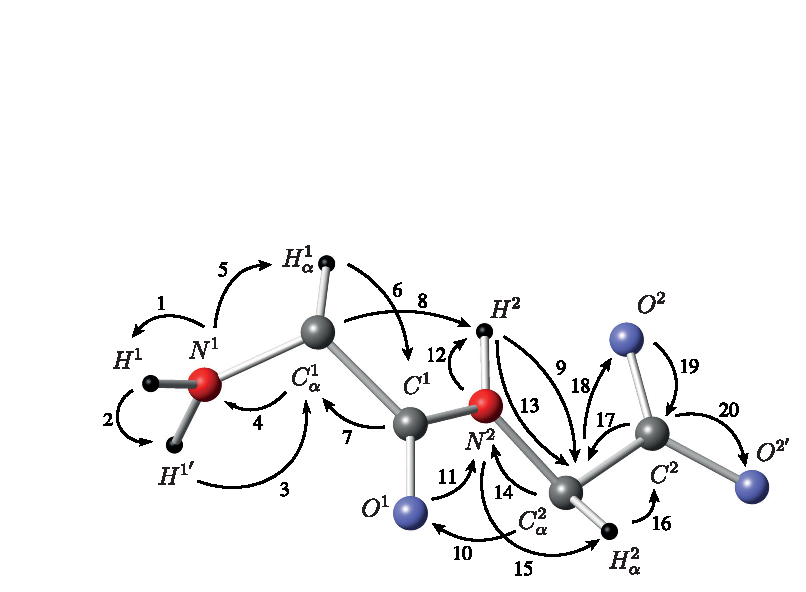
\includegraphics[width=0.65\linewidth]{proteinOrdened.eps}	
			\end{center}
		}	
	\end{frame}
	
	\section{HCProt}
	
	\begin{frame}
		\frametitle{\normalsize HCProt} 
		{
			\small
			
			Software para preprocessamento de instâncias PDB, chamado HCProt. 
			\begin{itemize}
				\item HCProt\footnote{https://github.com/caomem/PDBReader}: com ferramentas visuais para facilitar a criação de ordenações manuais.
				\item HCProtCLI\footnote{https://github.com/caomem/HCProtCLI}: interface linha de comando para a automação do preprocessamento;
			\end{itemize}
			
			\begin{center}
				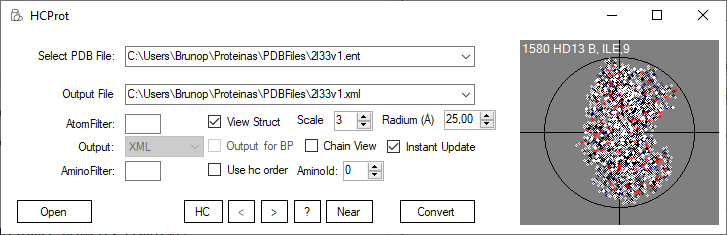
\includegraphics[width=0.8\linewidth]{molproj.png}	
			\end{center}
		}	
	\end{frame}
	
	\section{Referências}
	%Slide refe
	\begin{frame}		
		
		{\footnotesize
		\bibliographystyle{unsrt}
		\bibliography{references}}
	\end{frame}
	
	%Slide End
	\begin{frame}
		\begin{center}
			\vspace{1.5cm}
			Obrigado!\\
			\hspace{-4.5cm}
			
\includegraphics[scale=0.2]{logo.png}
			
			\vspace{-2.7cm}
			\hspace{5.5cm}
			
\includegraphics[scale=0.038]{logo_ufsc.png}
			
			\vspace{0.5cm}
			Contato: g.philippi\@grad.ufsc.br\\ UFSC - Blumenau
		\end{center}
	\end{frame}
	
\end{document}